CTU.SignBridge treats research validity as a machine-checkable property of the artifacts. A completed training process is eligible for reporting only when its identity, dataset, split, processing, source, runtime, and checkpoint provenance can be verified. Fig.~\ref{fig:pipeline} traces those artifacts and the two gates each run has to clear.

\begin{figure}[tbp]
\centering
% Portrait diagram: at 0.56\linewidth it stood 9.8cm tall, half the text
% block. 0.52 keeps the node labels legible and returns ~0.7cm.
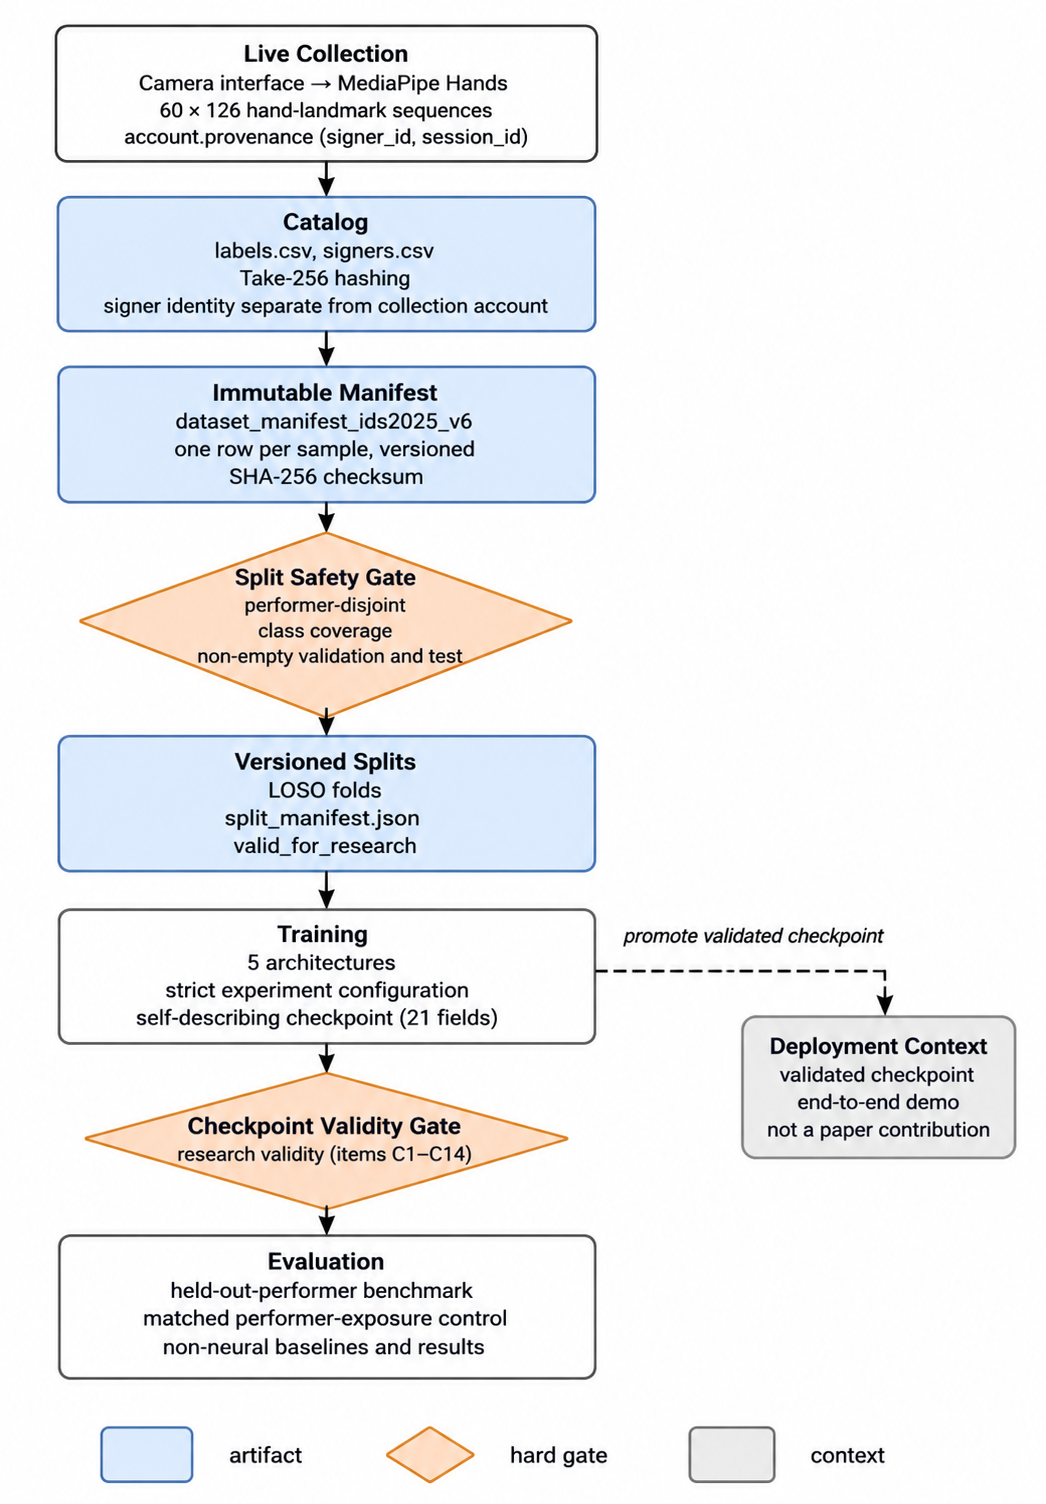
\includegraphics[
    width=0.52\linewidth,
    trim=8mm 5mm 8mm 5mm,
    clip
]{Figures/Figure1_pipeline.png}
\caption{Artifact-versioned CTU.SignBridge pipeline. Research results
are produced only after the split and checkpoint validity gates pass;
the deployment branch is shown only as system context.}
\label{fig:pipeline}
\end{figure}

\subsection{Identity, Manifest, and Split Artifacts}

Three things that are easy to conflate are kept apart in the identity catalog: the collection account, the canonical physical performer (\texttt{signer\_id}), and the recording session (\texttt{session\_id}). Separating them handles the problem in both directions, one account standing for several people and one person appearing under several historical identifiers. Every performer-disjoint check runs against the canonical physical-person mapping.

Class names need the same care. The vocabulary catalog defines profile-specific class identifiers, display labels, and storage slugs, and the slugs are Telex-style and vocabulary-aware so that two classes do not collide once Vietnamese diacritics are stripped.

Each processed sample is then indexed by an immutable manifest recording its profile, class, performer, available session provenance, storage reference, and processing contracts. A SHA-256 checksum binds that manifest to versioned train--validation--test splits and to every checkpoint downstream of them. When we correct an inventory we version it; we do not overwrite the previous one.

The split gate is where all of this becomes enforceable. It rejects unresolved identities, physical-performer overlap, missing class coverage, empty validation or test partitions, and labels outside the active profile. The fold counts show the gate doing its work: Hòa Đê admits four complete held-out-performer folds, while fingerspelling admits only F01 and F02 as complete 23-class test folds.

\subsection{Processing and Augmentation Contracts}

Training is bound to explicit preprocessing and augmentation versions; the experiments reported here use \texttt{v2\_wrist\_centered\_mirror}. An earlier version mirrored horizontally in image coordinates, after the sequence had already been wrist-centered:
\begin{align}
\text{v1, incorrect:}\quad x' &= 1-x, \label{eq:mirror_v1}\\
\text{v2, corrected:}\quad x' &= -x. \label{eq:mirror_v2}
\end{align}
Applied uniformly, Eq.~\eqref{eq:mirror_v1} does preserve pairwise distances, which is why it survived casual inspection. It nonetheless breaks the contract twice over: it shifts the origin away from the wrist, and it maps zero-valued missing-hand slots onto nonzero coordinates, so an absent hand becomes a hand at $x'=1$.

Reflecting about the wrist instead, as in Eq.~\eqref{eq:mirror_v2}, fixes both. We follow it by exchanging the left- and right-hand slots; missing slots stay at zero. The corrected contract passed 22 checks with no failures, covering wrist-origin, distance, span, empty-slot, padding, mask, involution, valid-frame, and coordinate-range properties. Temporal masking is disabled, since zero already means both ``missing hand'' and ``padding''.

\subsection{Self-Describing Checkpoints and Validity Gates}

A research checkpoint carries 21 required fields. They describe the model structure and input dimensions, the profile-specific label map, the dataset and split versions, the manifest checksum, the processing contracts, the seed and training configuration, the source revision and runtime environment, and finally how the checkpoint was selected and what it scored.

Every run is marked \texttt{smoke\_test} or \texttt{research}, and the default is \texttt{smoke\_test}, so a run has to earn the research label rather than inherit it. An early batch of 60 completed executions lacked sufficient provenance under this rule. We rejected all 60 and repeated them under the research protocol rather than patching metadata in after the fact, which would have defeated the purpose of recording it.

The post-training gate then checks 14 criteria: run purpose, required fields, artifact compatibility, manifest agreement, split validity, profile-label consistency, environment provenance, checkpoint restoration, nonempty test data, and successful completion. A run that cannot establish its validity is excluded.

\subsection{Deterministic Execution and Aggregation}

Strict execution fixes the Python, NumPy, and PyTorch seeds, deterministic PyTorch and cuDNN behavior, CUDA workspace settings, split artifacts, dataset ordering, and \texttt{num\_workers=0}. Only checkpoints that clear both the split gate and the research-validity gate reach aggregation. The public artifact package will carry code, weights, schemas, checksums, metrics, audit scripts, and environment metadata. Participant-level sequences stay private.